\documentclass{article}
\usepackage[utf8]{inputenc}
\usepackage{physics}
\usepackage{amsmath}
\usepackage{showlabels}
\usepackage{amssymb}
\title{Statistical Computing for Scientists and Engineers\\[1em] Homework 4}
\author{Jiale Shi}
\date{Oct/29/2018}

\usepackage{natbib}
\usepackage{graphicx}
\usepackage{array}
\begin{document}
\maketitle

\newpage
\section{Accept-Reject}
Generate samples of a standard normal distribution, $f(x) \sim N(0,1)$, using the accept-reject method with a double-exponential proposal distribution, $g(x|\alpha) = (\alpha/2)\exp(-\alpha |x|)$.

(a) Derive the upper bound for the likelihood ratio, $M=f(x)/g(x)$ and show that the ideal acceptance rate is obtained when $\alpha=1$

Solution:
a standard normal distribution, $f(x) \sim N(0,1)$

\begin{equation}
    f(x|0,1) = \frac{1}{\sqrt{2\pi}}\exp(-\frac{x^2}{2})
\end{equation}

\begin{equation}
    M = \frac{f(x)}{g(x)} = \frac{\frac{1}{\sqrt{2\pi}}\exp(-\frac{x^2}{2})}{(\alpha/2)\exp(-\alpha |x|)} = \frac{\sqrt{2}}{\alpha \sqrt{\pi}} \exp{-\frac{|x|^2}{2}+\alpha |x|}
\end{equation}

The ratio $M$ is max at $|x|=\alpha$.

\begin{equation}
    M =  \frac{\sqrt{2}}{\alpha \sqrt{\pi}} \exp{\frac{\alpha^2}{2}}
\end{equation}

\begin{equation}
\begin{aligned}
    &\pdv{M}{\alpha} = \frac{\sqrt{2}}{\sqrt{\pi}} \exp{\frac{\alpha^2}{2}} (1-\frac{1}{\alpha^2}) = 0 \\
    & \alpha = 1, M' = \frac{\sqrt{2}}{\sqrt{\pi}} \exp{\frac{1}{2}}
\end{aligned}
\end{equation}

(b) Implement the accept-reject method and plot the true PDF and the proposal distribution for $\alpha=1$ super-imposed on to the normalized histogram of your samples.

Solution:

$\alpha = 1$ and 
$M' = \frac{\sqrt{2}}{\sqrt{\pi}} \exp{\frac{1}{2}}$
    
\begin{figure}[h!]
\centering
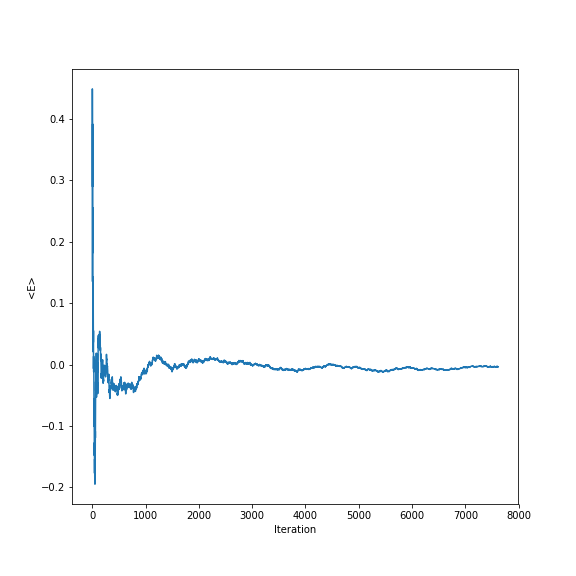
\includegraphics[scale=0.4]{h4p1b1.png}
\caption{$<E>$- iteration for $\alpha = 1$}
%\label{fig:universe}
\end{figure}

\begin{figure}[h!]
\centering
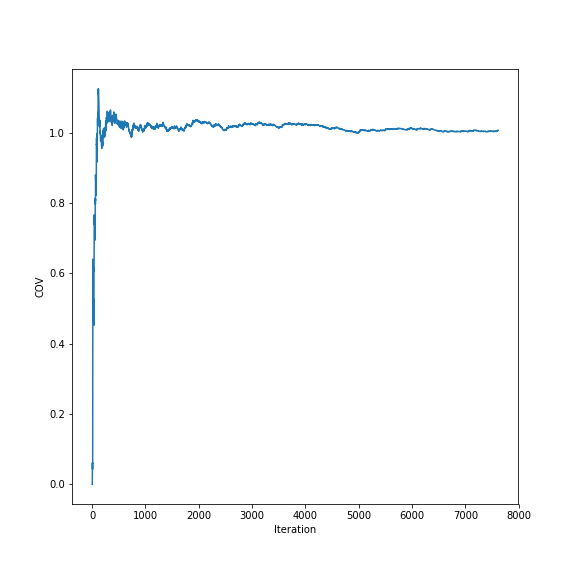
\includegraphics[scale=0.4]{h4p1b2.png}
\caption{COV- iteration for $\alpha = 1$}
%\label{fig:universe}
\end{figure}

\begin{figure}[h!]
\centering
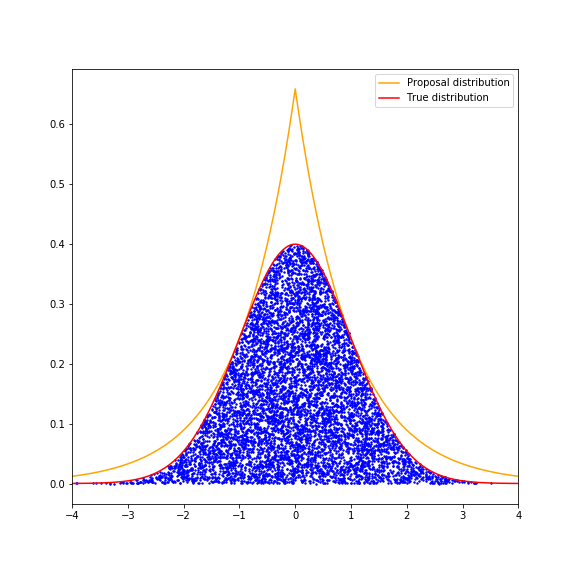
\includegraphics[scale=0.4]{h4p1b3.png}
\caption{ the true pdf and the proposal distribution for $\alpha = 1$}
%\label{fig:universe}
\end{figure}

\begin{figure}[h!]
\centering
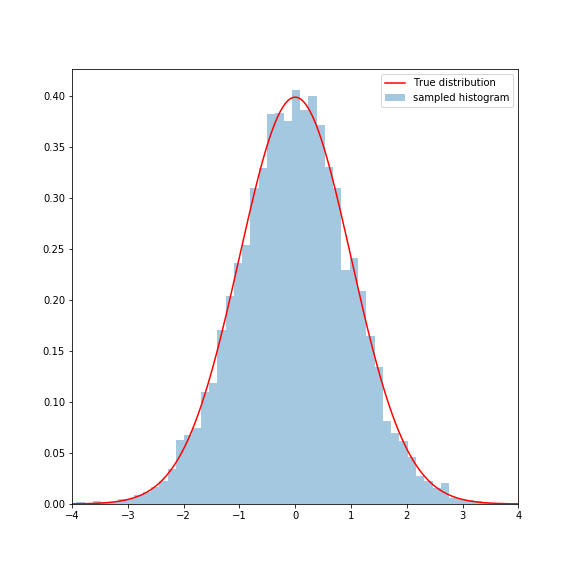
\includegraphics[scale=0.4]{h4p1b4.png}
\caption{histogram of samples for $\alpha = 1$}
%\label{fig:universe}
\end{figure}

\newpage
(c) Repeat part (b) but now use a sub-optimal proposal distribution with $\alpha=2$, plot both distributions and your histogram. How do the acceptance rates compare?

Solution:

$\alpha = 2$ and 
$M' = \frac{\sqrt{2}}{2\sqrt{\pi}} \exp{2}$
    
\begin{figure}[h!]
\centering
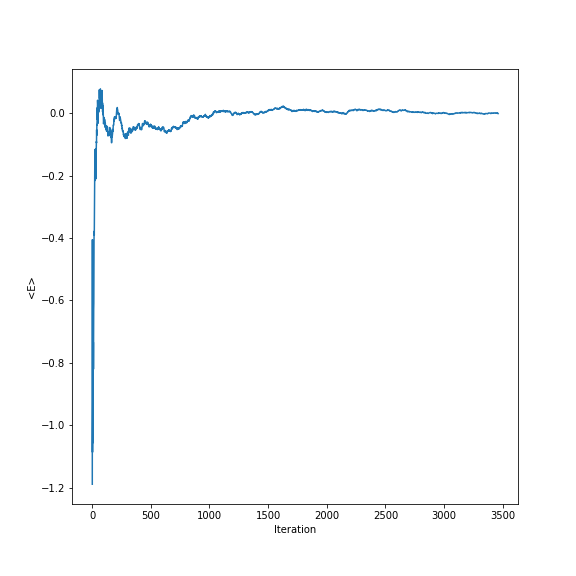
\includegraphics[scale=0.4]{h4p1c1.png}
\caption{$<E>$- iteration for $\alpha = 1$}
%\label{fig:universe}
\end{figure}

\begin{figure}[h!]
\centering
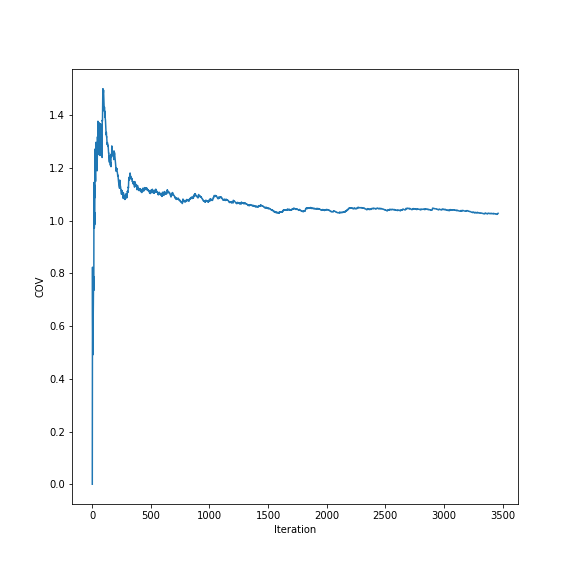
\includegraphics[scale=0.4]{h4p1c2.png}
\caption{COV- iteration for $\alpha = 1$}
%\label{fig:universe}
\end{figure}

\begin{figure}[h!]
\centering
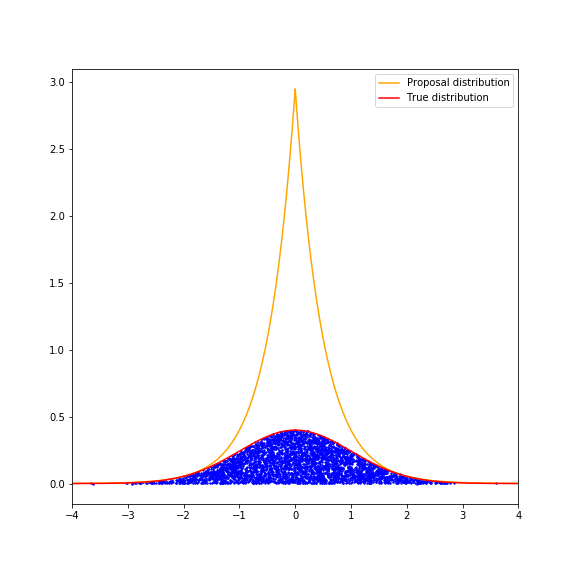
\includegraphics[scale=0.4]{h4p1c3.png}
\caption{ the true pdf and the proposal distribution for $\alpha = 1$}
%\label{fig:universe}
\end{figure}

\begin{figure}[h!]
\centering
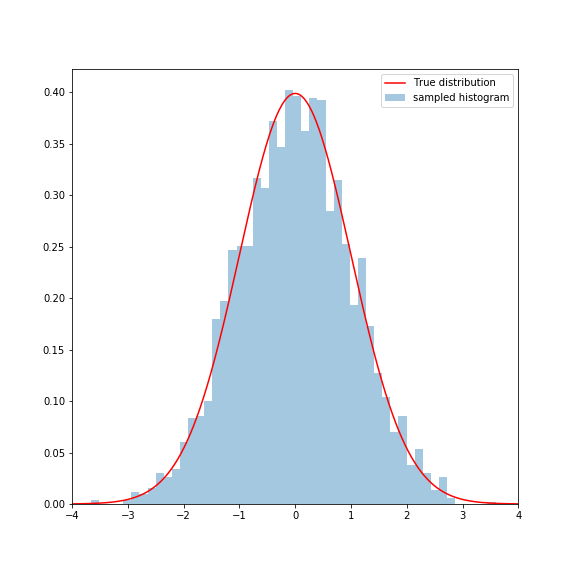
\includegraphics[scale=0.4]{h4p1c4.png}
\caption{histogram of samples for $\alpha = 1$}
%\label{fig:universe}
\end{figure}

By comparing Figure 1 and Figure 3, it is easy to figure out that the acceptance rates ($\alpha =2$) is smaller than that acceptance rates ($\alpha =1$)

\newpage
\section{Independent Metropolis-Hastings}
Traditionally in the Metropolis-Hastings algorithm the arbitrary proposal distribution is conditioned on the current state of the chain. Namely, one draws samples from $x' \sim q(x'|x_{t})$ where $x_t$ indicates the state of the chain. Consider a proposal distribution that is independent of the chain's current state $q(x')$. When such a distribution is used, this is referred to as the \textit{Independent Metropolis-Hasting algorithm}.

Prove that the Independent Metropolis-Hastings accepts more than the Accept-Reject method when both have identical target ($f(x')$) and proposal ($g(x')$) distributions.

Solution:

for Accept-Reject method:
\begin{equation}
\begin{aligned}
    & prob_{AJ} = \frac{f(x')}{M \cdot g(x')} \\
    & M = sup \frac{f(x)}{g(x)} \geq \frac{f(x)}{g(x)} 
\end{aligned}
\end{equation}
Since $M \cdot g(x') \geq f(x')$, $M \cdot g(x')$ curve is above $f(x')$ curve, $prob_{AJ} \leq 1$

for Metropolis-Hasting algorithm
\begin{equation}
\begin{aligned}
     & prob_{MH} = \min [1,\frac{\frac{f(x')}{g(x')}}{\frac{f(x_t)}{g(x_t)}}]  \\ %\geq \frac{f(x')}{M \cdot g(x')} \\
    & if  1 \leq \frac{\frac{f(x')}{g(x')}}{\frac{f(x_t)}{g(x_t)}} \to prob_{MH}=1 \geq prob_{AJ} \\
    & if  1 \geq \frac{\frac{f(x')}{g(x')}}{\frac{f(x_t)}{g(x_t)}} \to prob_{MH}=\frac{\frac{f(x')}{g(x')}}{\frac{f(x_t)}{g(x_t)}} \geq \frac{f(x')}{M \cdot g(x')} = prob_{AJ}
\end{aligned}
\end{equation}

The prob of Accept-Reject method is smaller than that of Metropolis-Hasting algorithm.
Therefore,the Independent Metropolis-Hastings accepts more than the Accept-Reject method when both have identical target ($f(x')$) and proposal ($g(x')$) distributions.


\newpage
\section{Accept-Reject $\&$ Metropolis-Hastings}
(a) Implement the accept-reject algorithm to calculate the mean of a gamma distribution $\mathcal{G}(4.3,6.2)$ using a $\mathcal{G}(4,7)$ candidate. Draw the true density function on top of the sample histogram and plot the convergence.

\begin{figure}[h!]
\centering
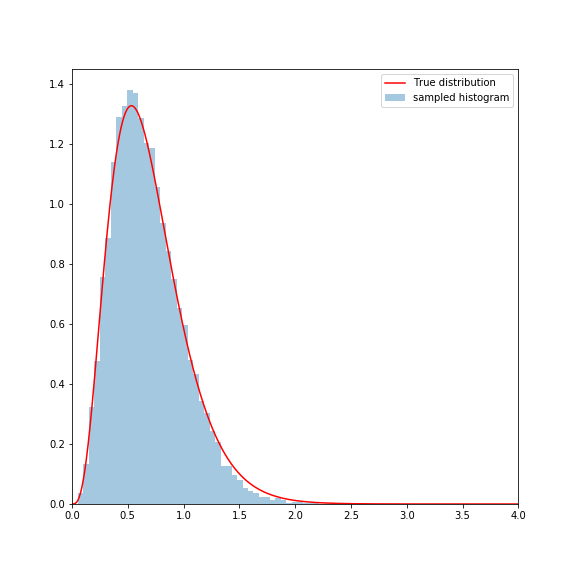
\includegraphics[scale=0.35]{h4p3a4.png}
\caption{ the true pdf and histogram of samples for accept-reject}
%\label{fig:universe}
\end{figure}

\begin{figure}[h!]
\centering
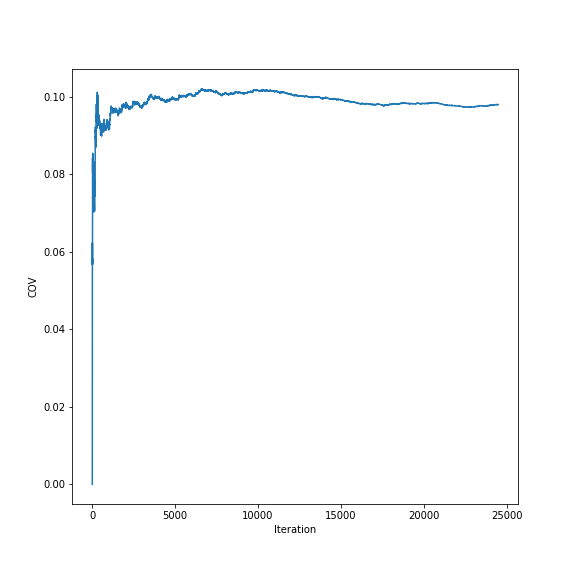
\includegraphics[scale=0.35]{h4p3a2.png}
\caption{ COV for accept-reject}
%\label{fig:universe}
\end{figure}

\newpage
(b) Implement the Metropolis-Hastings algorithm to calculate the mean of a gamma distribution $\mathcal{G}(4.3,6.2)$ using the following candidate densities:

A gamma $\mathcal{G}(4,7)$ candidate distribution.

A gamma $\mathcal{G}(5,6)$ candidate distribution.

For both candidate distributions draw the true and candidate density functions on top of 
the sampled histogram. Plot the convergence using each candidate distribution on the same axis . How do the means compare?

\begin{figure}[h!]
\centering
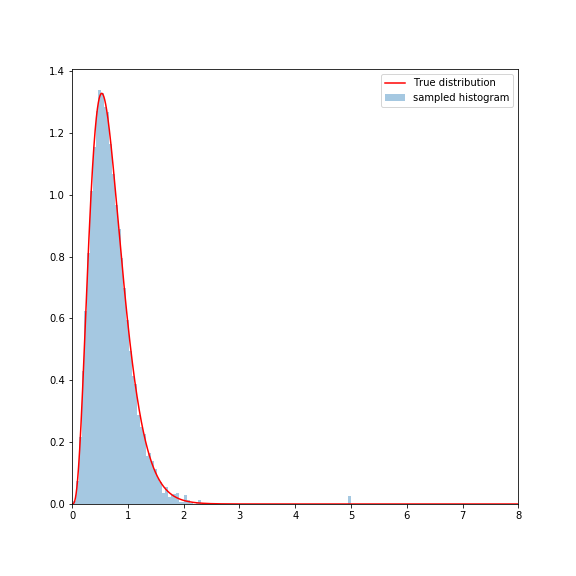
\includegraphics[scale=0.3]{h4p3b13.png}
\caption{ $\mathcal{G}(4,7)$}
%\label{fig:universe}
\end{figure}

\begin{figure}[h!]
\centering
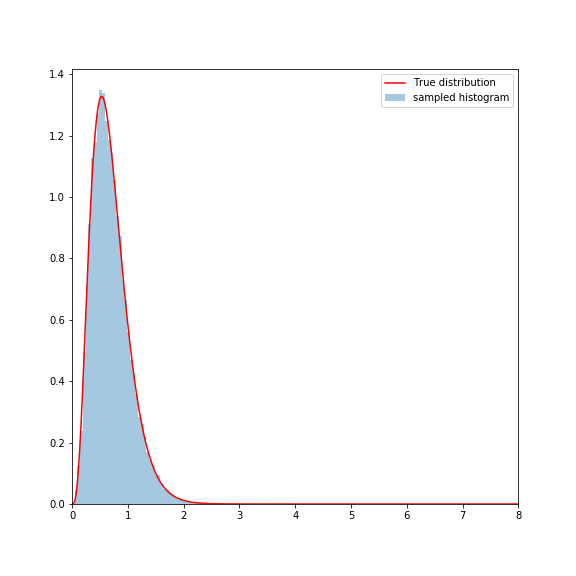
\includegraphics[scale=0.3]{h4p3b23.png}
\caption{ $\mathcal{G}(5,6)$}
%\label{fig:universe}
\end{figure}

\begin{figure}[h!]
\centering
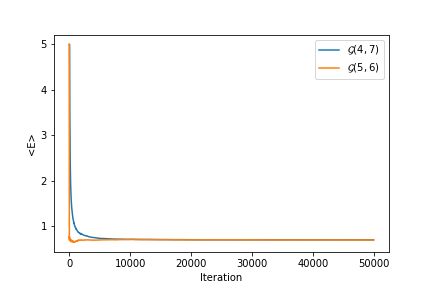
\includegraphics[scale=0.45]{h4p3bEcompare.png}
\caption{ $<E>$ comparation for different proposal functions}
%\label{fig:universe}
\end{figure}

\begin{figure}[h!]
\centering
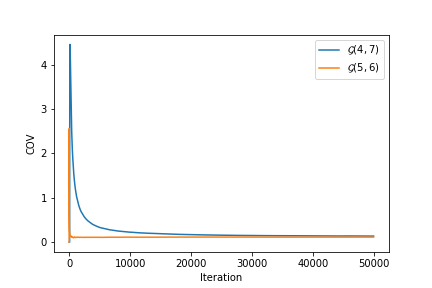
\includegraphics[scale=0.45]{h4p3bCOVcompare.png}
\caption{ COV comparation for different proposal functions}
%\label{fig:universe}
\end{figure}

$\mathcal{G}(5,6)$ convergences much quickly than $\mathcal{G}(4,7)$. And we can see it from COV-iteration and $<E>$-iteration figures.
\\
\\
\\
\\
\\
\\
\\
\\
\\
\\
\\
\\
\\
\\
\\

\section{Gibbs $\&$ Metropolis-Hastings}
Consider sampling from a 2D Gaussian. Suppose $x \sim \mathcal{N}(\mu, \Sigma) $ where $\mu = (1,1)$ and $\Sigma = (1,-0.5;-0.5,1)$.

(a) Derive the full conditional $p(x_1 | x_2)$ and $p(x_2 | x_1)$. Implement the Gibbs algorithm for this case and plot the 1D marginals $p(x_1)$ and $p(x_2)$ as well as (superimposed) the computed histograms.

Derive the full conditional distribution from Bishop-Pattern Recognition and Machine Learning(2.81 and 2.82)
\begin{equation}
\begin{aligned}
\mu_{a|b} = \mu_{a} + \Sigma_{ab}\Sigma_{bb}^{-1}(x_{b}-\mu_{b})
\end{aligned}
\end{equation}

\begin{equation}
\begin{aligned}
\Sigma_{a|b} = \Sigma_{aa} -\Sigma_{ab}\Sigma_{bb}^{-1}\Sigma_{ba}
\end{aligned}
\end{equation}

Therefore,

\begin{equation}
\begin{aligned}
& \mu_{x_1|x_2} = 1 -0.5(x_{2}-1) \\
& \Sigma_{x_1|x_2} = 0.75 \\
& x_1|x_2 \sim \mathcal{N}(1 -0.5(x_{2}-1), 0.75) \\
& \mu_{x_2|x_1} = 1 -0.5(x_{1}-1) \\
& \Sigma_{x_2|x_1} = 0.75 \\
& x_2|x_1 \sim \mathcal{N}(1 -0.5(x_{1}-1), 0.75) \\
\end{aligned}
\end{equation}

\begin{figure}[h!]
\centering
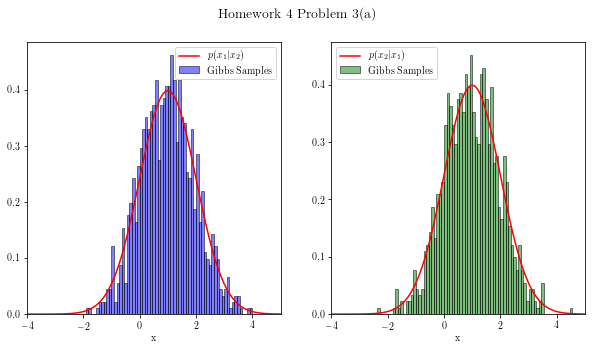
\includegraphics[scale=0.45]{HW4P41.png}
\caption{ }
%\label{fig:universe}
\end{figure}

(b) Let us now consider block-wise Metropolis Hastings. For our proposal distribution, $q(x)$ let us  use a normal centered at the previous state/sample of the Markov chain/sampler, i.e: $q(x|x^{(t-1)}) \sim N(x^{(t-1)}, I)$, where I is a 2D identity matrix. Show the 2D target distribution and its sampled approximation.

\begin{figure}[h!]
\centering
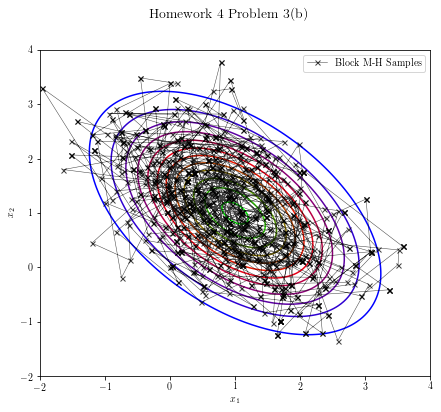
\includegraphics[scale=0.45]{HW4P42.png}
\caption{ }
%\label{fig:universe}
\end{figure}

(c) We now consider component-wise Metropolis Hastings approximation of the same problem. The proposal distribution $q(x)$ is now a univariate Normal distribution with unit variance in the direction of the i-th dimension to be sampled. Show the sampled and exact target distribution.
Show your results and compare the convergence with that obtained with the block-wise, component-wise Metropolis-Hastings and Gibbs implementation.

\begin{figure}[h!]
\centering
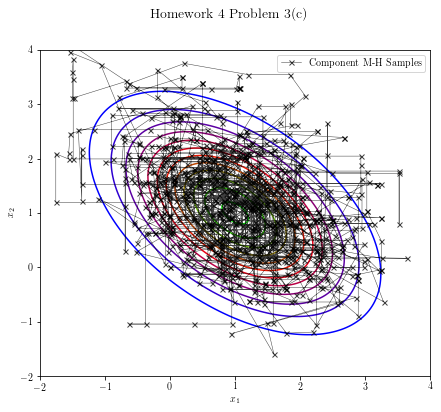
\includegraphics[scale=0.45]{HW4P43.png}
\caption{}
%\label{fig:universe}
\end{figure}

Compare the convergence with that with that obtained with the block-wise, component-wise Metropolis-Hastings and Gibbs implementation.

\begin{figure}[h!]
\centering
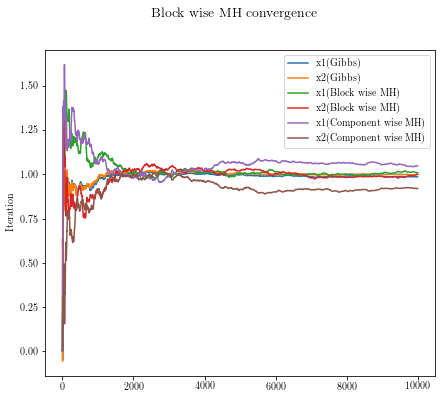
\includegraphics[scale=0.45]{HW4P44.png}
\caption{$<E>$ convergence}
%\label{fig:universe}
\end{figure}

\begin{figure}[h!]
\centering
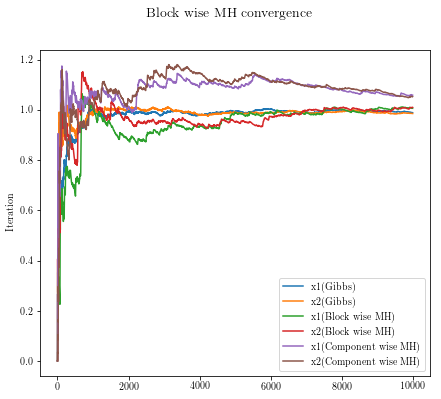
\includegraphics[scale=0.45]{HW4P45.png}
\caption{COV convergence}
%\label{fig:universe}
\end{figure}

From $<E>$ convergence and COV convergence, it is easy to find that 
the convergence rate: Gibbs is the fastest, Block-wise MH is the second, component-wise is the slowest.

\newpage
\section{Metropolis-Hastings}
Consider the braking data of Tukey. It corresponds to breaking distances $y_{i,j}$ of cars driving at speeds $x_{i}$. It is thought that a good model for this dataset is quadratic model:
\begin{equation}
    y_{i,j} = \beta_{0} +\beta_{1}x_{i} + \beta_{2}x_{i}^{2}+\epsilon_{i,j}
\end{equation}
where $\epsilon_{i,j} \sim  N(0,\sigma^2), i=1, ..., k$ and $j=1,...,n_{i}$
If we assume that $\epsilon_{i,j} \sim  N(0,\sigma^2)$ are independent, then the likelihood function is 
\begin{equation}
    (\frac{1}{\sigma^2})^{N/2} e^{-\frac{1}{2\sigma^2}\sum_{i,j}(y_{i,j}-\beta_{0}-\beta_{1}x_{i} - \beta_{2}x_{i}^{2})}
\end{equation}
We can view this likelihood as a posterior distribution of $\beta_{0},\beta_{1},\beta_{2},\sigma^2$ and we can sample from it with a Metropolis-Hasting algorithm.

(a) Obtain maximum likelihood estimate for $\beta_{0}$, $\beta_{1}$, $\beta_{2}$, $\sigma^{2}$
\begin{equation}
    I(\beta_{0},\beta_{1},\beta_{2},\sigma^2 | y,X ) =  (\frac{1}{\sigma^2})^{N/2} e^{-\frac{1}{2\sigma^2}\sum_{i,j}(y_{i,j}-\beta_{0}-\beta_{1}x_{i} - \beta_{2}x_{i}^{2})}
\end{equation}
take the log of $I$
\begin{equation}
    \log I(\beta_{0},\beta_{1},\beta_{2},\sigma^2 | y,X) = (N/2) \log(\frac{1}{\sigma^2}) -\frac{1}{2\sigma^2}\sum_{i,j}(y_{i,j}-\beta_{0}-\beta_{1}x_{i} - \beta_{2}x_{i}^{2})
\end{equation}

for $\beta_{0}$, $\beta_{1}$, $\beta_{2}$:
\begin{equation}
\begin{aligned}
    & \frac{\partial I}{\partial \beta_{0}} = 0;\\
    & \frac{\partial I}{\partial \beta_{1}} = 0;\\
    & \frac{\partial I}{\partial \beta_{2}} = 0;\\
    & \frac{\partial I}{\partial \sigma} = 0;
\end{aligned}
\end{equation}
then
\begin{equation}
\begin{aligned}
    & \sum_{i,j} y_{i,j} = \sum_{i} n_{i}(\beta_{0}+\beta_{1}x_{i}+\beta_{2}x_{i}^{2});\\
    & \sum_{i,j} y_{i,j} x_{i} = \sum_{i} n_{i}(\beta_{0}+\beta_{1}x_{i}+\beta_{2}x_{i}^{2}) x_{i};\\
    & \sum_{i,j} y_{i,j} x_{i}^{2} = \sum_{i} n_{i}(\beta_{0}+\beta_{1}x_{i}+\beta_{2}x_{i}^{2})x_{i}^{2};\\
    & \sigma^2 = \frac{1}{N}\sum_{i,j}(y_{i,j}-\beta_{0}-\beta_{1}x_{i} - \beta_{2}x_{i}^{2})
\end{aligned}
\end{equation}

We call
\begin{equation}
\begin{aligned}
& Y = [y_{1,1},...,y_{1,n_{1}},y_{2,1},...,y_{k,1},...,y_{k,n_{k}}] \\
& X = [x_{1}I_{(n_{1} \times 1)},...,x_{k}I_{(n_{k}\times 1)}]
\end{aligned}
\end{equation}

The solution of $\beta$ satisfying those equation has a closed form:
\begin{equation}
    \hat{\beta} = ([I,X,X^2]^{T}[I,X,X^2])^{-1}[I,X,X^2]^{T} Y
\end{equation}

for $\sigma^2$, put estimated $\hat{\beta}$ into the likelihood expression of $\sigma^{2}$.
\begin{equation}
     \hat{\sigma}^2 = \frac{1}{N}\sum_{i,j}(y_{i,j}-\hat{\beta}_{0}-\hat{\beta}_{1}x_{i} - \hat{\beta}_{2}x_{i}^{2})
\end{equation}

Use the braking data of Tukey,
MLE of beta is $\hat{\beta} = [2.47 0.91 0.1]^{T}$; MLE of sigma is $\sigma^2 = 216.5$.

(b) Use the estimates to select a candidate distribution. Take normal for $\beta_{0}$, $\beta_{1}$, $\beta_{2}$, and inverted Gamma for $\sigma^{2}$.

The MLE estimated $\hat{\beta}$ can be used as the mean parameter of normal proposal density for $\beta$ because it is unbiased estimator. As for the variance parameter in proposal density, we can rely on its covariance matrix approximation.

\begin{equation}
    \mathbb{V} (\beta) | X,\sigma^2) = ([I,X,X^2]^{T}[I,X,X^2])^{-1} \hat{\sigma}^{2} 
\end{equation}

The proposal density for $\beta$ is then
\begin{equation}
    \beta \sim N(\hat{\beta}, \mathbb{V} (\beta|X,\sigma^2))
\end{equation}

For the proposal density of parameters $\sigma^2$, according to Cochran's theorem:
\begin{equation}
    \frac{N \hat{\sigma}^2}{\sigma^2} \sim \mathcal{X}_{N-3}^2 = \mathcal{G}(\frac{N-3}{2},2) \to \frac{1}{\sigma^2} \sim  \mathcal{G}(\frac{N-3}{2},\frac{2}{N\hat{\sigma}^2})
\end{equation}

Therefore, the final proposal density for $\beta, \sigma$ is then
\begin{equation}
\begin{aligned}
    p(\beta, \sigma^2) &= \mathcal{N}(\beta| \hat{\beta}, \mathbb{V}(\beta|X,\sigma^2)) \mathcal{IG}(\sigma^2|\frac{N-3}{2},\frac{2}{N\hat{\sigma}^2}) \\
    & = \mathcal{N}([2.47,0.91,0.1],\left[ \begin{array}{ccc}
206.37 & -27.22 & 0.821 \\
-27.22 & 3.89 & -0.124 \\
0.821 & -0.124 & 0.0041
\end{array} \right]) \mathcal{IG}(23.5,5405)
\end{aligned}
\end{equation}

For student T distribution
\begin{equation}
    \mathbb{V} (\beta) | X,\sigma^2) = ([I,X,X^2]^{T}[I,X,X^2])^{-1} \hat{\sigma}^{2} \frac{v}{v-2} 
\end{equation}
This covariance is bigger than the previous one.

\begin{equation}
\begin{aligned}
    p(\beta, \sigma^2) &= \mathcal{N}(\beta| \hat{\beta}, \mathbb{V}(\beta|X,\sigma^2)) \mathcal{IG}(\sigma^2|\frac{N-3}{2},\frac{2}{N\hat{\sigma}^2}) \\
    & = \mathcal{N}([2.47,0.91,0.1],\left[ \begin{array}{ccc}
412.74 & -54.44 & 1.642 \\
-54.44 & 7.78 & -0.248 \\
1.642 & -0.248 & 0.0082
\end{array} \right]) \mathcal{IG}(23.5,5405)
\end{aligned}
\end{equation}

(c) Make histogram of the posterior distributions of the parameters. Monitor convergence.

Robustness considerations could lead to using an error distribution with heavier tails. If we assume that $\epsilon_{i,j} \sim Gamma(0,\sigma^{2})$ independent, then the likelihood function is 

\begin{equation}
    (\frac{1}{\sigma^2})^{N/2} \prod_{i,j} (1+\frac{1}{v} \frac{(y_{i,j}-\beta_{0}-\beta_{1}x_{i}-\beta_{2}x_{i}^{2})^2}{\sigma^2})^{(v+1)/2}
\end{equation}

where $v$ is the degrees of freedom. For $v=4$, use Metropolis-Hastings to sample  $\beta_{0}$, $\beta_{1}$, $\beta_{2}$, $\sigma^{2}$ from the posterior distribution. Use either normal or $\Gamma$ candidates for $\beta_{0}$, $\beta_{1}$, $\beta_{2}$ and inverted Gamma or half-$\Gamma$ for $\sigma^2$.

\begin{figure}[h!]
\centering
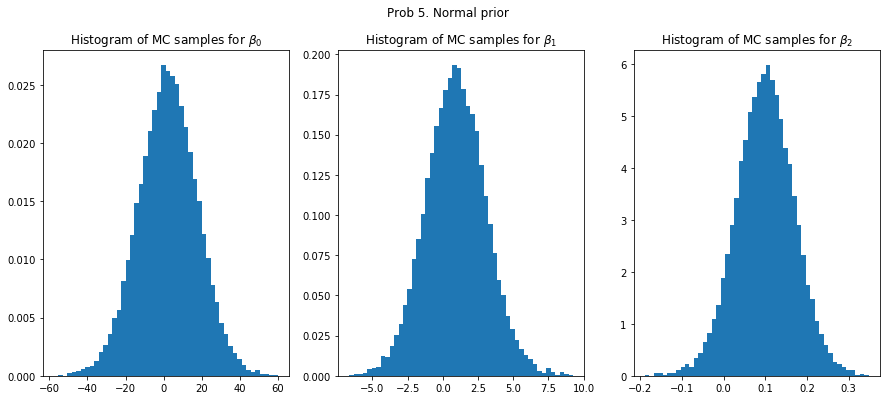
\includegraphics[scale=0.45]{HW4P51.png}
\caption{$\beta$ Normal distribution}
%\label{fig:universe}
\end{figure}

\begin{figure}[h!]
\centering
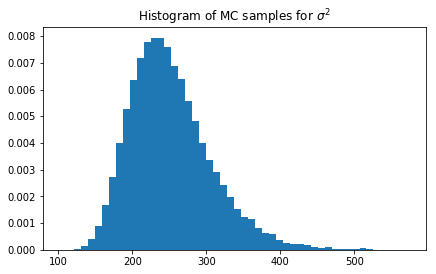
\includegraphics[scale=0.45]{HW4P52.png}
\caption{$\sigma$ Normal distribution}
%\label{fig:universe}
\end{figure}

\begin{figure}[h!]
\centering
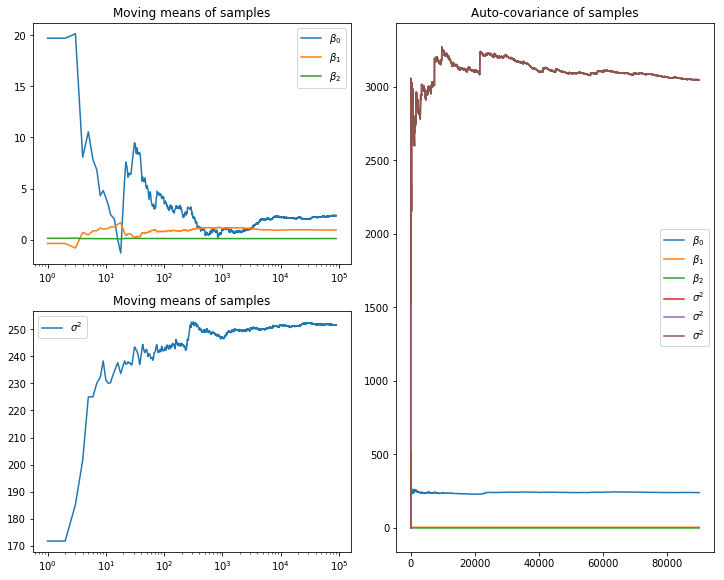
\includegraphics[scale=0.45]{HW4P53.png}
\caption{Normal distribution}
%\label{fig:universe}
\end{figure}

\begin{figure}[h!]
\centering
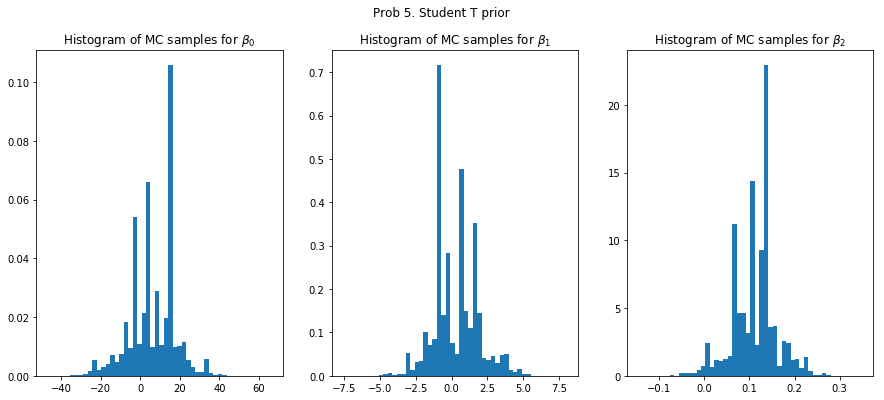
\includegraphics[scale=0.45]{HW4P54.png}
\caption{$\beta$ Student T distribution}
%\label{fig:universe}
\end{figure}

\begin{figure}[h!]
\centering
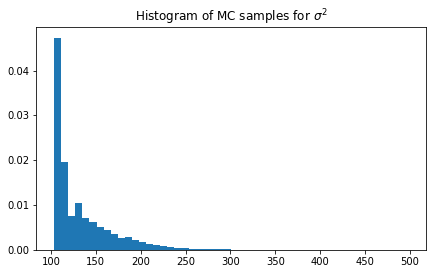
\includegraphics[scale=0.45]{HW4P55.png}
\caption{$\sigma$ Student T distribution}
%\label{fig:universe}
\end{figure}

\begin{figure}[h!]
\centering
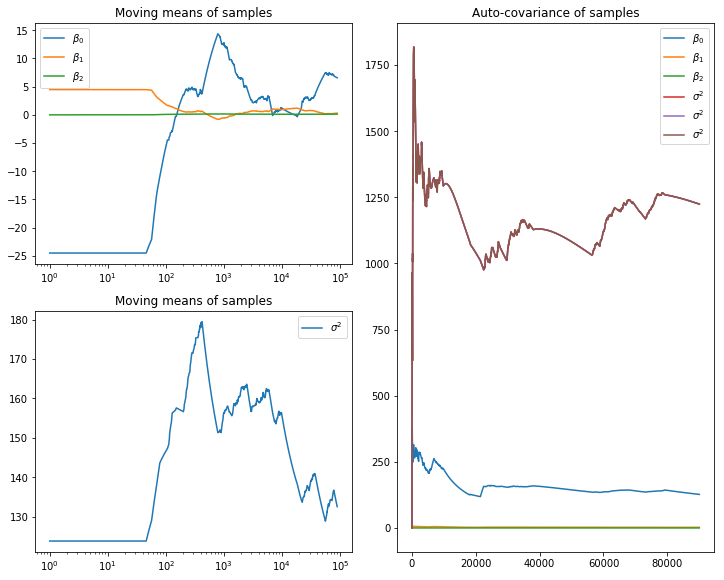
\includegraphics[scale=0.45]{HW4P56.png}
\caption{Student T distribution}
%\label{fig:universe}
\end{figure}

Normal distribution candidate is better than student T distribution candidate.
%\bibliographystyle{plain}
%\bibliography{references}
\end{document}
